\documentclass[conference]{IEEEtran}
\usepackage[utf8]{inputenc}

\IEEEoverridecommandlockouts

\usepackage{cite}
\usepackage{amsmath,amssymb,amsfonts}
\usepackage{algorithmic}
\usepackage{graphicx}
\usepackage{textcomp}
\usepackage{xcolor}
\usepackage{multirow}
\usepackage{tikz}
\usetikzlibrary{positioning}
\def\checkmark{\tikz\fill[scale=0.4](0,.35) -- (.25,0) -- (1,.7) -- (.25,.15) -- cycle;}
\usepackage{svg}
\usepackage{listings}

%colours
\definecolor{pastelblue1}{HTML}{B0D0D3} % Powder Blue
\definecolor{pastelblue2}{HTML}{C7D2FE} % Periwinkle Mist
\definecolor{pastelblue3}{HTML}{D4E8F4} % Sky Whisper
\definecolor{pastelblue4}{HTML}{A8C5DA} % Arctic Haze
\definecolor{pastelblue5}{HTML}{C3CFE2} % Frosted Indigo

\addtolength{\topmargin}{+0.1cm} 

\lstdefinelanguage{json}{
    basicstyle=\ttfamily\footnotesize,
    breaklines=true,
    morestring=[b]",
    morecomment=[l]{//},
}

\begin{document}

\title{Network Identity Management: Application, Action and Device Aware Monitoring }

\author{\IEEEauthorblockN{Cenab Batu Bora}
\IEEEauthorblockA{\textit{Faculty of Computing Science} \\
\textit{University of Alberta}\\
Edmonton, Canada \\
cenab@ualberta.ca}
\and
\IEEEauthorblockN{Julia Silva Weber}
\IEEEauthorblockA{\textit{Faculty of Computer Science} \\
\textit{Dalhousie University}\\
Halifax, Canada \\
julia.weber@dal.ca}
\and
\IEEEauthorblockN{Nur Zincir-Heywood}
\IEEEauthorblockA{ \textit{Faculty of Computer Science} \\
\textit{Dalhousie University}\\
Halifax, Canada \\
zincir@cs.dal.ca}
}

\maketitle



\begin{abstract}
Instant Message Applications (IMAs) are often used in sensitive environments, where they pose a significant risk of accidental policy breaches or security lapses. To address these risks, this paper introduces Network Identity Management (NIM), a set of techniques specifically designed for such high-risk applications. NIM provides a novel approach that enables network-layer, identity-aware access control for encrypted applications. To support NIM, we introduce techniques to establish the essential visibility layer. These techniques use machine learning (ML) to analyze encrypted traffic metadata. The ML models are trained on data produced by our scalable, cloud-native Android traffic generation framework. Our ML framework accurately identifies: (1) the application in use, (2) the specific user action being performed, and (3) the originating device—using only encrypted traffic metadata from multi-user environments. For its primary task, our method, using emulated traffic from eight Instant Messaging Applications (IMAs), yielded a 98.6\% F1-score for application identification with Gradient Boosting. Additionally, the method demonstrated near-perfect device identification based exclusively on encrypted traffic metadata. Furthermore, supplementary experiments provide initial validation for user action classification (group vs. one‑on‑one messaging), achieving a 73.3\% F1-score in distinguishing between group chats and direct messages using environment-agnostic patterns. 
\end{abstract}

\begin{IEEEkeywords}
Encrypted traffic analysis, instant messaging applications, AI/ML, network identity management 
\end{IEEEkeywords}

\section{Introduction}
The use of powerful, encrypted mobile applications, often on employee-owned devices (BYOD), is widespread in enterprise and government networks. However, organizations must ensure their secure and compliant use to prevent accidental data leakage or unauthorized user actions. Crucially, this must be achieved while upholding user privacy and the security benefits provided by end-to-end encryption. Traditional policy enforcement methods relying on firewalls, domain blocking, and traffic inspection are incompatible with modern encryption standards. Consequently, practical solutions like the proposed Network Identity Management (NIM) are required. NIM is designed to infer key activities—such as the application being used, its device of origin, and the nature of the action (like a video call or group chat)—based on network behavior. Based on this visibility, NIM can enforce granular, predefined permission levels or policies. For instance, it can restrict access to certain applications or high-risk features based on user roles. These enforcement actions rely solely on communication patterns and information from encrypted traffic. This methodology represents a significant advancement over current measures, which are often ineffective or overly restrictive.

NIM is conceptualized as a network-layer Identity and Access Management system for encrypted applications. NIM facilitates context-aware access decisions through a deliberate sequence: it first validates user identity and then permits network access to particular applications, a methodology akin to Role-Based Access Control. In this framework, NIM defines access groups based on organizational roles and then assigns permissions for specific applications or resources to these groups. When a device connects, it becomes associated with a user's identity and their designated access group(s). The fundamental technical challenge for NIM lies in reliably identifying the application solely from encrypted traffic data.

Our method analyzes encrypted traffic metadata to identify the active application and its source device. Furthermore, by exclusively leveraging environment-agnostic structural patterns, our method differentiates specific communication features, such as successfully classifying group chats versus direct messages. Our results confirm the feasibility of identifying, at the network level, granular information such as 'User A's device is using Signal for group messaging.'

The ability of our models to distinguish between chat types suggests that other user actions, such as file transfers or voice calls, are also likely to produce unique traffic signatures. Action identification could indeed enhance selective blocking with more granularity. However, the principal contribution of our application and device identification is to enable robust application-level access control via NIM.

Our work lays the foundation for this vision, offering three key contributions:
\begin{itemize}
    \item \textbf{Introduce ML-based tracing of user actions, applications, and devices in encrypted traffic}: We demonstrate an ML-based method for visibility into encrypted network traffic, achieving high accuracy in detecting user actions, identifying IMAs, and determining originating devices from metadata. This enables proactive, identity-driven NIM and Zero Trust principles.
    \item \textbf{Architect a cloud-native traffic-generation framework}: We implemented a scalable cloud-native emulation framework for generating diverse mobile application traffic datasets without sensitive live user data, crucial for developing and validating NIM capabilities.
    \item \textbf{Simulate realistic user behaviors in traffic generation}: Our framework simulates asynchronous conversations and natural group chat patterns, creating detailed traffic signatures for training ML models to distinguish applications and devices, demonstrating the feasibility of our metadata-based identification for NIM.
\end{itemize}

The remainder of this paper is organized as follows. Section II reviews encrypted traffic analysis and group chat classification. Section III details our framework, traffic generation and feature extraction. Section IV evaluates performance across ML models, and Section V discusses conclusions and future work.

\section{Related Work}
In their study, Erdenebaatar et al.\cite{b1} utilized Machine Learning (ML) in conjunction with an Android Studio virtual machine to analyze network traffic from six IMAs. Their analysis encompassed synchronous and asynchronous text-based communications. The framework developed by Erdenebaatar et al. automates IMA traffic generation, capture, and flow-level analysis of network activities.

Abiodun et al. \cite{b4} employed an enhanced honey encryption scheme to reinforce the security of IMA systems and to confound the time and resources of malicious actors. Although their experiments aimed to reinforce security in IMAs, testing was confined to private conversations, thereby excluding group chat scenarios. 

Shapira et al. \cite{b8} introduced a novel approach for encrypted Internet traffic classification, capable of both categorizing traffic types and identifying specific applications, based solely on time and size related features. However, the authors do not specify whether the datasets they created involved private or group chats. Their dataset is publicly available \cite{b13}. They reported an average classification accuracy of 89.3\% for chat IMAs.

Li, Zhida, et al. \cite{b16} explored the efficacy of various fast ML models including Gaussian Naive Bayes, K-Nearest Neighbors, Decision Tree, Random Forests, Extra-Trees, and XGBoost and evaluated on F1-Score. Their analysis guided our selection of ML models.

%Shahraki et al. \cite{b9} reviewed data stream processing tools and frameworks for online data processing. Their review discussed the pros and cons of these tools and their compatibility with commonly used data processing frameworks. 

In comparison with previous works, our research explores traffic signatures for asynchronous and group chat communications of different IMAs in a virtual machine setting. We extend the work of Erdenebaatar et al.\cite{b1} by focusing on group chats involving more than two users rather than one-to-one user communication. Moreover, we design and develop a cloud-based virtual infrastructure to scale up user behavior emulation; we also increased the number of IMAs used and improved traffic capturing techniques. 

\section{Methodology}
\subsection{Experimental Objectives}
This study aims to:

\begin{itemize}
    \item \textbf{Develop a User Behavior Emulation and Traffic Generation Framework}: Emulate and generate encrypted traffic for eight IMAs reflecting realistic group conversational patterns (asynchronous messaging, multi-device participation, variable group sizes).
    \item \textbf{Train Machine Learning Models for Identification, Classification, and Action Tracing}: Train ML models for network-level user tracking, mapping encrypted traffic to IMAs, actions, and devices using flow-level metadata, laying groundwork for identifying feature-specific traffic patterns.
\end{itemize}

Our codebase and dataset are publicly available to ensure reproducibility on GitHub/Zenodo\footnote{https://doi.org/10.5281/zenodo.15460189} and IEEE DataPort\footnote{https://dx.doi.org/10.21227/rmg3-b562}.

\subsection{Emulation \& Traffic Generation Framework}\label{AA}
\begin{figure}[!ht]
    \centering
    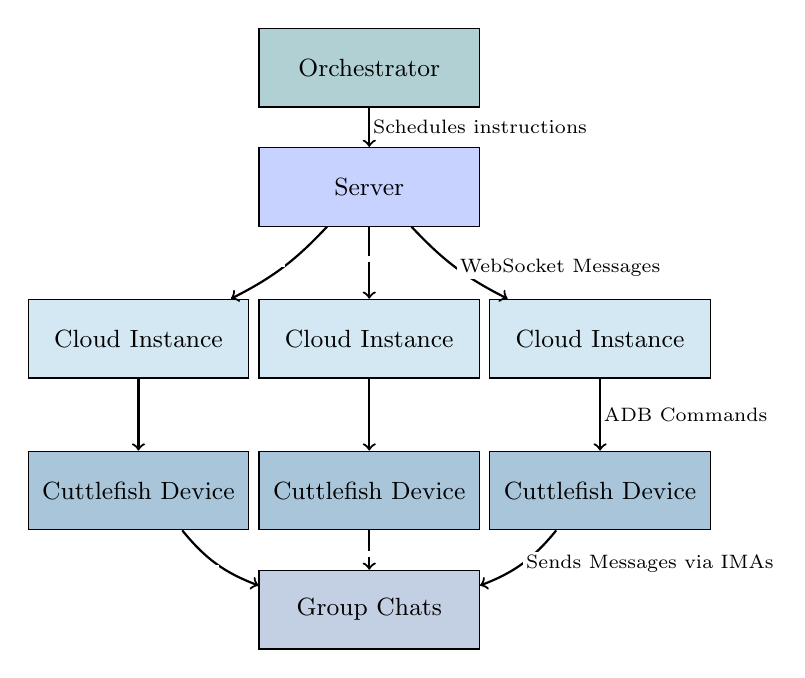
\begin{tikzpicture}[
        node distance=1.4cm and 2.2cm,
        every node/.style={font=\small},
        block/.style={rectangle, draw, minimum width=2.8cm, minimum height=1cm, align=center},
        layer/.style={rectangle, draw=none, minimum height=0.5cm},
        line/.style={->, thick},
        textnode/.style={font=\scriptsize, midway, fill=white, inner sep=1pt}
    ]

        % Server
        \node[block, fill=pastelblue1] (orchestrator) {Orchestrator};
        \node[block, fill=pastelblue2, below=0.5cm of orchestrator] (server) {Server};

        % Clients
        \node[layer, below=0.3cm of server] (clientslabel) {};
        \node[block, fill=pastelblue3, below left=0.1cm and 1.4cm of clientslabel] (instance1) {Cloud Instance};
        \node[block, fill=pastelblue3, below=0.1cm of clientslabel] (instance2) {Cloud Instance};
        \node[block, fill=pastelblue3, below right=0.1cm and 1.4cm of clientslabel] (instance3) {Cloud Instance};

        % Traffic Capture
        \node[layer, below=0.3cm of instance2] (trafficlabel) {};
        \node[block, fill=pastelblue4, below left=0.1cm and 1.4cm of trafficlabel] (device1) {Cuttlefish Device};
        \node[block, fill=pastelblue4, below=0.1cm of trafficlabel] (device2) {Cuttlefish Device};
        \node[block, fill=pastelblue4, below right=0.1cm and 1.4cm of trafficlabel] (device3) {Cuttlefish Device};

        % Group Chats
        \node[block, fill=pastelblue5, below=0.5cm of device2] (groupchats) {Group Chats};

        % Arrows from Orchestrator to Server
        \draw[line] (orchestrator) -- node[textnode, right] {Schedules instructions} (server);
        
        % Arrows from Orchestrator to Instances
        \draw[line] (server) to[bend left=10] node[textnode, above] {} (instance1);
        \draw[line] (server) -- node[textnode, above] {} (instance2);
        \draw[line] (server) to[bend right=10] node[textnode, right] {WebSocket Messages} (instance3);

        % ADB Commands from Instances to Devices
        \draw[line] (instance1) -- node[textnode, left] {} (device1);
        \draw[line] (instance2) -- node[textnode, left] {} (device2);
        \draw[line] (instance3) -- node[textnode, right] {ADB Commands} (device3);

        % IMAs arrows to Group Chats
        \draw[line] (device1) to[bend right=15] node[textnode, below] {} (groupchats);
        \draw[line] (device2) -- node[textnode, below] {} (groupchats);
        \draw[line] (device3) to[bend left=15] node[textnode, right] {Sends Messages via IMAs} (groupchats);

    \end{tikzpicture}
    \caption{Experiment architecture overview}
    \label{fig:architecture}
\end{figure}
The end-to-end architecture for generating encrypted group chat traffic is illustrated in Figure \ref{fig:architecture}. Our system utilizes three Google Cloud instances running Ubuntu 20.04 LTS to emulate Android smartphones using Android Cuttlefish\footnote{Each instance is provisioned with 2 vCPUs, 13 GB RAM, and 400 GB SSD storage.}. These Cuttlefish instances host eight IMAs.

An orchestration framework governs message delivery across the emulated environment. On each emulated device (client), Operating System level commands, such as sending messages or switching applications, are executed via the ADB. A server manages message timing and IMA selection. This server also synchronizes conversations across all devices through WebSocket connections.

We use tcpdump to capture encrypted traffic, producing PCAP files for later analysis. Our system's cloud-native architecture inherently supports horizontal scalability, allowing for the on-demand provisioning of additional devices to simulate larger groups, thereby eliminating hardware dependencies.

For the purpose of this study, asynchronous chat is defined as a multi-user interaction. Such interactions are characterized by irregular, delayed replies that do not adhere to strict timing or sequencing. To replicate the dynamics of real-world group chats, our framework generates asynchronous conversations. These conversations are designed to mirror human behavior across various devices and IMAs.

The system leverages publicly available datasets of natural dialogue. From these datasets, it assigns dialogue lines to specific devices and IMAs. This process incorporates randomized wait times, ranging from 15 to 60 seconds, as detailed in Table \ref{tab:Top5TrimmedDialogue}. This randomization effectively mimics the irregular pacing of actual conversations. For instance, it accommodates longer pauses for complex replies and allows for shorter gaps during quick responses. To further emulate the brevity of mobile chats, messages are limited to the first 50 characters.
Furthermore, the framework captures the multi-platform spontaneity inherent in real group interactions. It achieves this by distributing dialogues across multiple IMAs; for example, a debate might initiate in Teams and subsequently continue in Telegram.

Although the current study focuses on general chat activity adequate for IMA identification, future iterations will need to address a broader scope. Specifically, they will necessitate generating traffic associated with distinct actions within each IMA, such as voice call initiation, file uploading, or video streaming.

\begin{table}[!ht]
\centering
\caption{dialogue schedule snippet}
\label{tab:Top5TrimmedDialogue}
\resizebox{0.9\columnwidth}{!}{%
\begin{tabular}{|l|c|c|c|}
\hline
\multicolumn{1}{|c|}{\textbf{Dialogue}} & \textbf{Device} & \textbf{IMA} & \textbf{Wait Time (seconds)} \\ \hline
Nay, answer me. ...                      & 3              & signal       & 45                          \\ \hline
He. ...                                  & 2              & signal       & 60                          \\ \hline
You come most ...                        & 3              & teams        & 55                          \\ \hline
Not a mouse ...                          & 3              & skype        & 58                          \\ \hline
Well, good night. ...                    & 1              & signal       & 33                          \\ \hline
\multicolumn{4}{|c|}{\textit{... conversation continues ...}} \\ \hline
\end{tabular}%
}
\end{table}

\subsection{Traffic Orchestration and Client-Device Interaction}
An orchestrator, running on the server, manages device-specific message queues. This management prevents bottlenecks by efficiently scheduling messages derived from the emulated dialogue data. Once the message schedule is determined, the orchestrator performs several actions. First, it establishes a WebSocket connection. Then, it declares the number of Cuttlefish devices expected to connect. Finally, it relays messages to these devices according to the schedule. As each Cuttlefish device registers with the server via its WebSocket connection, the server assigns it a unique numeric ID. Subsequently, the server routes the appropriate messages to that specific device in real time.

On the client side, each Cuttlefish device operates under the control of a dedicated script. This script is responsible for receiving commands from the server. It then executes these commands using the Android Debug Bridge (ADB). The commands issued by the server direct the Cuttlefish devices to emulate user interactions. These interactions, such as taps, swipes, and keyboard input, are performed according to predefined scripts. Consequently, each device actively sends text messages to group chats within multiple IMAs. The devices also automatically switch among these applications, simulating realistic multi-application usage patterns. 

\subsection{Traffic Capture and Labeling}
First, encrypted traffic is captured using the \texttt{tcpdump} utility. This captured traffic is subsequently isolated. The isolation process utilizes dynamic filters, which are generated from \texttt{netstat} logs. These \texttt{netstat} logs are collected at 60-second intervals. Next, these logs undergo processing. They are transformed into a JSON-structured session database. This database records specific details for each IMA, including associated ports, IP addresses, and activity timestamps. For example, an entry might indicate port \texttt{51558} was active between UNIX epochs \texttt{1726056090 and 1726057619}. To achieve precise traffic isolation, the following methodologies are then applied:

\begin{itemize}
    \item \textbf{Time-Bounded Port/IP Correlation}: Matches active ports/IPs from \texttt{netstat} logs (e.g., \texttt{192.168.97.2:59895 → 52.157.5.65:443}) with timestamps for session-aware filters (e.g., Teams call on port \texttt{51558} isolated during active windows).
    \item \textbf{TLS SNI Disambiguation}: Resolves port conflicts (e.g., Slack/WhatsApp on 443) by extracting SNI fields from TLS ClientHello packets (e.g., \texttt{*.signal.org} for Signal).
    \item \textbf{Application-Aware IP Whitelisting}: Identifies IMAs using known static IP ranges (e.g., Telegram's \texttt{51.81.11.66}), bypassing ephemeral port limitations.
\end{itemize}

\begin{lstlisting}[
    language=,  % Remove "json" - this is Wireshark filter syntax
    basicstyle=\ttfamily\footnotesize,
    breaklines=true,
    caption={Hypothetical Hybrid Wireshark filter combining time windows, IP whitelisting, and SNI validation for Discord.},
    label={lst:wireshark}
]
((tcp.port == 51558 AND  // Discord sessions
   frame.time_epoch >= 1726056090 AND 
   frame.time_epoch <= 1726057619) OR
  (tcp.port == 51558 AND 
   frame.time_epoch >= 1726126204 AND 
   frame.time_epoch <= 1726127414) OR
  (ip.addr == 51.81.11.66 OR ip.addr == 51.81.47.120) OR  // Discord IP ranges
  (tls.handshake.extensions_server_name contains "discord.org"))  // Discord SNI
\end{lstlisting}

\textbf{Filter Breakdown in Listing \ref{lst:wireshark}:}
\begin{itemize}
    \item Lines 1-4: Isolates Discord traffic on port \texttt{51558} during two recorded session windows.
    \item Line 5: Tags Discord traffic using its known IP addresses recorded.
    \item Lines 6 onwards: Validates Discord traffic via SNI fields, resolving HTTPS/443 ambiguity.
\end{itemize}

After isolation of traffic, traffic flows are extracted using Tranalyzer2 \footnote{https://tranalyzer.com/} before labeling network traffic with the corresponding IMA. Tranalyzer2 determines 109 features, representing a broad range of traffic characteristics.

\subsection{Apps and Device Multi-classification}
To identify both the IMAs and the source device, we first performed feature selection on the 109 extracted traffic attributes. Techniques such as mutual information and the ANOVA F-value were used to filter out the most relevant features, while hierarchical clustering with dendrograms helped reduce dimensionality.

Next, we applied a multi-output approach, allowing simultaneous prediction of the IMA label and the originating device. We used scikit-learn\footnote{https://scikit-learn.org} for most of our algorithms. However, some models, like Support Vector Machines, were computationally intensive and took over 40 hours to train on a CPU using our dataset. To accelerate this process, we employed the GPU-accelerated cuML\footnote{https://rapids.ai/} library for these models.

We evaluated each model's performance using accuracy, precision, recall, and F1-score, and further analyzed results with confusion matrices. A 10-fold cross-validation was conducted to gauge the models' consistency, capturing both average performance and potential worst-case scenarios.

\subsection{Distinguishing the User Actions (Group vs. 1:1 Chat)}
We conducted a binary classification experiment to differentiate between group chats and 1:1 chats. The goal was to see if intrinsic traffic patterns could distinguish these communication types, which is important for creating granular NIM policies. We used a combined dataset comprising direct messaging traffic data from Erdenebaatar et al.\cite{b1} and the group chat traffic data we generated (Section III-B/C) aiding the model in identifying fundamental structural differences.

Our feature engineering focused on distilling core communication patterns thought to be inherent to the interaction type, rather than the network environment. We calculated relational ratios (e.g., sent/received bytes/packets) reflecting conversational balance, used normalized timing features (e.g., inter-arrival times) to capture relative pacing, and developed structural indicators of message flow, independent of absolute network speeds or latencies. Conversely, we excluded low-level TCP metrics (e.g., `tcpSeqSntBytes`, `tcpWinSzChgDirCnt`). We did this because these metrics are often heavily influenced by network conditions rather than the communication pattern itself. Therefore, they would be less reliable for a practical NIM system that needs to operate across varied environments.

We evaluated several ML algorithms for classification, including those used for application/device identification (Section III-F). Gradient Boosting provided the best performance in differentiating group vs. 1:1 chats based on these distilled patterns. Structured cross-validation and dimensionality reduction were used throughout the evaluation to confirm that classification relied on meaningful behavioral patterns, suitable for reliable NIM decisions.

\section{Evaluation and Results}
\subsection{Dataset and Traffic Characteristics}
As demonstrated by our results, this scalable approach successfully produced 37 hours of encrypted group chat traffic that closely mirrors real-device performance—even across eight IMAs, with consistent flow characteristics and sufficient variability to train our ML models. As shown in Table \ref{tab:flowExtraction}, Slack had the highest data volume (36.33 MB per device) and Teams produced the most flows (4,052 on Device 1). Device 1 consistently generated 15–20\% more traffic than Devices 2/3, likely due to the randomized emulated conversations (Section III-C).


\subsection{Feature Selection and Impact}
ANOVA F-value analysis (Table \ref{tab:TP}) identified critical features for distinguishing IMAs without decrypting messages: \begin{enumerate} 
    \item \textbf{tcpMSS}: Differentiates Discord and Slack. 
    \item \textbf{ipMaxdIPID}: Flags Signal, Skype, and Telegram. 
    \item \textbf{tcpMinWinSz}: Highlights bulk transfers in Skype and Teams. 
\end{enumerate} 
These features are fundamental to our ML framework, directly enabling both application and device-level identification and providing foundational support for tasks such as tracing malicious activity.

\begin{table}[!ht]
\centering
\caption{IMA Anova F-Value Top 5 Features}
\label{tab:TP}
\resizebox{\columnwidth}{!}{%
\begin{tabular}{|l|c|c|c|}
\hline
\multicolumn{1}{|c|}{\textbf{Rank}} & \textbf{Feature} & \textbf{\begin{tabular}[c]{@{}c@{}}Normalized \\ F-Score\end{tabular}} & \textbf{Description} \\ \hline
1 & tcpMSS & 1.000 & \begin{tabular}[c]{@{}c@{}}Max bytes in a single TCP segment.\end{tabular} \\ \hline
2 & ipMaxdIPID & 0.578 & \begin{tabular}[c]{@{}c@{}}Max IP ID delta between packets.\end{tabular} \\ \hline
3 & ipMinTTL & 0.576 & \begin{tabular}[c]{@{}c@{}}Minimum TTL observed in IP packets.\end{tabular} \\ \hline
4 & dstPort & 0.569 & \begin{tabular}[c]{@{}c@{}}Destination port number.\end{tabular} \\ \hline
5 & tcpMinWinSz & 0.568 & \begin{tabular}[c]{@{}c@{}}Smallest TCP window size.\end{tabular} \\ \hline
\end{tabular}%
}
\end{table}

\begin{table}[!ht]
\centering
\caption{IMA flow extraction information}
\label{tab:flowExtraction}
\resizebox{\columnwidth}{!}{%
\begin{tabular}{|l|l|c|c|c|}
\hline
                              & \multicolumn{1}{c|}{\textbf{IMA}} & \textbf{\# of Packets} & \textbf{Total Size (Mb)} & \textbf{Total \# of Flows} \\ \hline
\multirow{8}{*}{Device 1} & Discord                           & 24878                 & 10                       & 612                        \\ \cline{2-5} 
                              & Messenger                         & 39891                 & 12                       & 1556                       \\ \cline{2-5} 
                              & RocketChat                        & 33680                 & 5                        & 499                        \\ \cline{2-5} 
                              & Slack                             & 107303                & 36                       & 1838                       \\ \cline{2-5} 
                              & Skype                             & 43825                 & 28                       & 2261                       \\ \cline{2-5} 
                              & Signal                            & 54699                 & 10                       & 704                        \\ \cline{2-5} 
                              & Teams                             & 70473                 & 37                       & 4052                       \\ \cline{2-5} 
                              & Telegram                          & 23690                 & 5                        & 866                        \\ \hline
\multirow{8}{*}{Device 2} & Discord                           & 24767                 & 7                        & 631                        \\ \cline{2-5} 
                              & Messenger                         & 42945                 & 13                       & 1589                       \\ \cline{2-5} 
                              & RocketChat                        & 32583                 & 5                        & 406                        \\ \cline{2-5} 
                              & Slack                             & 113898                & 38                       & 1809                       \\ \cline{2-5} 
                              & Skype                             & 37218                 & 24                       & 1774                       \\ \cline{2-5} 
                              & Signal                            & 52069                 & 10                       & 824                        \\ \cline{2-5} 
                              & Teams                             & 59543                 & 31                       & 3448                       \\ \cline{2-5} 
                              & Telegram                          & 22958                 & 4                        & 812                        \\ \hline
\multirow{8}{*}{Device 3} & Discord                           & 23586                 & 6                        & 596                        \\ \cline{2-5} 
                              & Messenger                         & 34949                 & 11                       & 1477                       \\ \cline{2-5} 
                              & RocketChat                        & 35241                 & 5                        & 431                        \\ \cline{2-5} 
                              & Slack                             & 107275                & 35                       & 1791                       \\ \cline{2-5} 
                              & Skype                             & 32635                 & 22                       & 1673                       \\ \cline{2-5} 
                              & Signal                            & 53627                 & 10                       & 696                        \\ \cline{2-5} 
                              & Teams                             & 52754                 & 27                       & 3163                       \\ \cline{2-5} 
                              & Telegram                          & 23791                 & 4                        & 797                        \\ \hline
\end{tabular}%
}
\end{table}

\subsection{Measuring Success}
Tree-based methods (Decision Tree, Random Forest, Gradient Boosting) excel on the 109-feature dataset for IMA classification (Table \ref{tab:MinMaxeresults}). In particular, the Gradient Boosting model achieved an F1-score exceeding 97\%.

As demonstrated by our experimental results, our ML framework achieved a 98.6\% F1-score in distinguishing between eight IMAs, thereby confirming our goal of high-precision identification in complex, multi-user environments. A 10-fold cross-validation yielded a 98.6\% F1-score, and testing on a 20\% holdout subset achieved 97.8\%, confirming the robustness of our approach.

\begin{table*}[!ht]
\centering
\caption{Min-Max results}
\label{tab:MinMaxeresults} 
%\resizebox{\textwidth}{!}{%
\resizebox{15cm}{!}{%
\begin{tabular}{|l|ccc|ccc|ccc|}
\hline
\multicolumn{1}{|c|}{\multirow{2}{*}{\textbf{Model}}}            & \multicolumn{3}{c|}{\textbf{\begin{tabular}[c]{@{}c@{}}IMA Application\\ Classification\end{tabular}}}                                                                                                                                              & \multicolumn{3}{c|}{\textbf{Device Identification}}                                                                                                                                                                                              & \multicolumn{3}{c|}{\textbf{\begin{tabular}[c]{@{}c@{}}Group vs 1:1 user action\\ Classification\end{tabular}}}                                                                                                                      \\ \cline{2-10} 
\multicolumn{1}{|c|}{}                                           & \multicolumn{1}{l|}{\textit{Precision}}                                                & \multicolumn{1}{l|}{\textit{Recall}}                                                   & \multicolumn{1}{l|}{\textit{F1-Score}}                            & \multicolumn{1}{l|}{\textit{Precision}}                                               & \multicolumn{1}{l|}{\textit{Recall}}                                                  & \multicolumn{1}{l|}{\textit{F1-Score}}                           & \multicolumn{1}{l|}{\textit{Precision}}                                              & \multicolumn{1}{l|}{\textit{Recall}}                                        & \multicolumn{1}{l|}{\textit{F1-Score}}                          \\ \hline
\begin{tabular}[c]{@{}l@{}}Naive \\ Bayes\end{tabular}           & \multicolumn{1}{c|}{\begin{tabular}[c]{@{}c@{}}0.673 -\\  0.715\end{tabular}}          & \multicolumn{1}{c|}{\begin{tabular}[c]{@{}c@{}}0.720 - \\ 0.762\end{tabular}}          & \begin{tabular}[c]{@{}c@{}}0.647 - \\ 0.700\end{tabular}          & \multicolumn{1}{c|}{\begin{tabular}[c]{@{}c@{}}0.2304 - \\ 0.4321\end{tabular}}       & \multicolumn{1}{c|}{\begin{tabular}[c]{@{}c@{}}0.3335 - \\ 0.3596\end{tabular}}       & \begin{tabular}[c]{@{}c@{}}0.1998 - \\ 0.2656\end{tabular}       & \multicolumn{1}{c|}{\begin{tabular}[c]{@{}c@{}}0.254-\\ 0.888\end{tabular}}          & \multicolumn{1}{c|}{\begin{tabular}[c]{@{}c@{}}0.369-\\ 0.89\end{tabular}}  & \begin{tabular}[c]{@{}c@{}}0.301-\\ 0.889\end{tabular}          \\ \hline
\begin{tabular}[c]{@{}l@{}}Decision \\ Tree\end{tabular}         & \multicolumn{1}{c|}{\begin{tabular}[c]{@{}c@{}}0.964 -\\  0.975\end{tabular}}          & \multicolumn{1}{c|}{\begin{tabular}[c]{@{}c@{}}0.964 -\\  0.977\end{tabular}}          & \begin{tabular}[c]{@{}c@{}}0.965 -\\  0.975\end{tabular}          & \multicolumn{1}{c|}{\begin{tabular}[c]{@{}c@{}}0.9994 - \\ 1.0\end{tabular}}          & \multicolumn{1}{c|}{\begin{tabular}[c]{@{}c@{}}0.9994 -\\ 1.0\end{tabular}}           & \begin{tabular}[c]{@{}c@{}}0.9994 - \\ 1.0\end{tabular}          & \multicolumn{1}{c|}{\begin{tabular}[c]{@{}c@{}}0.274-\\ 0.878\end{tabular}}          & \multicolumn{1}{c|}{\begin{tabular}[c]{@{}c@{}}0.43-\\ 0.874\end{tabular}}  & \begin{tabular}[c]{@{}c@{}}0.335-\\ 0.876\end{tabular}          \\ \hline
\begin{tabular}[c]{@{}l@{}}Random \\ Forest\end{tabular}         & \multicolumn{1}{c|}{\begin{tabular}[c]{@{}c@{}}0.968 - \\ 0.977\end{tabular}}          & \multicolumn{1}{c|}{\begin{tabular}[c]{@{}c@{}}0.967 - \\ 0.977\end{tabular}}          & \begin{tabular}[c]{@{}c@{}}0.967 - \\ 0.977\end{tabular}          & \multicolumn{1}{c|}{\begin{tabular}[c]{@{}c@{}}0.9951 - \\ 0.9973\end{tabular}}       & \multicolumn{1}{c|}{\begin{tabular}[c]{@{}c@{}}0.9949 -\\  0.9974\end{tabular}}       & \begin{tabular}[c]{@{}c@{}}0.9950 - \\ 0.9973\end{tabular}       & \multicolumn{1}{c|}{\begin{tabular}[c]{@{}c@{}}0.266-\\ 0.905\end{tabular}}          & \multicolumn{1}{c|}{\begin{tabular}[c]{@{}c@{}}0.404-\\ 0.894\end{tabular}} & \begin{tabular}[c]{@{}c@{}}0.321-\\ 0.898\end{tabular}          \\ \hline
\begin{tabular}[c]{@{}l@{}}Gradient\\ Boosting\end{tabular}      & \multicolumn{1}{c|}{\textbf{\begin{tabular}[c]{@{}c@{}}0.977 - \\ 0.986\end{tabular}}} & \multicolumn{1}{c|}{\textbf{\begin{tabular}[c]{@{}c@{}}0.976 - \\ 0.985\end{tabular}}} & \textbf{\begin{tabular}[c]{@{}c@{}}0.976 - \\ 0.986\end{tabular}} & \multicolumn{1}{c|}{\textbf{\begin{tabular}[c]{@{}c@{}}0.9997 - \\ 1.0\end{tabular}}} & \multicolumn{1}{c|}{\textbf{\begin{tabular}[c]{@{}c@{}}0.9997 - \\ 1.0\end{tabular}}} & \textbf{\begin{tabular}[c]{@{}c@{}}0.9997 - \\ 1.0\end{tabular}} & \multicolumn{1}{c|}{\begin{tabular}[c]{@{}c@{}}0.275-\\ 0.909\end{tabular}} & \multicolumn{1}{c|}{\begin{tabular}[c]{@{}c@{}}0.435-\\ 0.903\end{tabular}} & \begin{tabular}[c]{@{}c@{}}0.337-\\ 0.905\end{tabular}          \\ \hline
%\begin{tabular}[c]{@{}l@{}}Logistic\\ Regression\end{tabular}    & \multicolumn{1}{c|}{\begin{tabular}[c]{@{}c@{}}0.935 - \\ 0.950\end{tabular}}          & \multicolumn{1}{c|}{\begin{tabular}[c]{@{}c@{}}0.945 -\\  0.960\end{tabular}}          & \begin{tabular}[c]{@{}c@{}}0.939 - \\ 0.954\end{tabular}          & \multicolumn{1}{c|}{\begin{tabular}[c]{@{}c@{}}0.4065 - \\ 0.4304\end{tabular}}       & \multicolumn{1}{c|}{\begin{tabular}[c]{@{}c@{}}0.4112 - \\ 0.4349\end{tabular}}       & \begin{tabular}[c]{@{}c@{}}0.4071 - \\ 0.4299\end{tabular}       & \multicolumn{1}{c|}{\begin{tabular}[c]{@{}c@{}}0.636-\\ 0.991\end{tabular}}          & \multicolumn{1}{c|}{\begin{tabular}[c]{@{}c@{}}0.615-\\ 0.992\end{tabular}} & \textbf{\begin{tabular}[c]{@{}c@{}}0.609-\\ 0.992\end{tabular}} \\ \hline
\begin{tabular}[c]{@{}l@{}}Support Vector\\ Machine\end{tabular} & \multicolumn{1}{c|}{\begin{tabular}[c]{@{}c@{}}0.695 - \\ 0.744\end{tabular}}          & \multicolumn{1}{c|}{\begin{tabular}[c]{@{}c@{}}0.750 -\\  0.768\end{tabular}}          & \begin{tabular}[c]{@{}c@{}}0.701 - \\ 0.729\end{tabular}          & \multicolumn{1}{c|}{\begin{tabular}[c]{@{}c@{}}0.2987 - \\ 0.3301\end{tabular}}       & \multicolumn{1}{c|}{\begin{tabular}[c]{@{}c@{}}0.3110 - \\ 0.3281\end{tabular}}       & \begin{tabular}[c]{@{}c@{}}0.2317 - \\ 0.2672\end{tabular}       & \multicolumn{1}{c|}{\begin{tabular}[c]{@{}c@{}}0.257-\\ 0.914\end{tabular}}          & \multicolumn{1}{c|}{\begin{tabular}[c]{@{}c@{}}0.376-\\ 0.917\end{tabular}} & \begin{tabular}[c]{@{}c@{}}0.305-\\ 0.915\end{tabular}          \\ \hline
\end{tabular}%
}
\end{table*}

 % HIGHLIGHT: COMMENTED OUT CONFUSION MATRIX
 % \begin{figure}[!ht]
 %     \centering
 %     \includegraphics[width=0.45\textwidth]{Figure_2.png}
 %     \caption{Gradient Boosting application confusion matrix}
 %     \label{fig:example}
 % \end{figure}

\subsection{Device Identification Results}
For device identification, we assigned three labels (Device1, Device2, Device3) and observed that tree-based algorithms again delivered the highest performance (Table \ref{tab:MinMaxeresults}). The Gradient Boosting model achieved near-perfect results in our 10-fold tests—with eight folds reaching 100\% F1-score and the remaining two folds above 99.9\%. These findings underscore our framework's ability to precisely map encrypted flows to specific devices, a critical aspect of our contribution. This precision is a critical prerequisite for real-world scenarios such as tracing and isolating malicious or compromised devices in complex group chat environments, all without decrypting message contents.

\begin{table*}[!ht]
\centering
\caption{Group vs 1:1 user action classification for each IMA app for \textbf{Gradient Boosting}}
\label{tab:MLDevresults} 
%\resizebox{\textwidth}{!}{%
\resizebox{10cm}{!}{%
\begin{tabular}{|l|c|c|c|c|}
\hline
\multicolumn{1}{|c|}{\textbf{IMA}} & \textbf{Accuracy} & \textbf{Precision} & \textbf{Recall} & \textbf{F1 Score} \\ \hline
\textbf{Discord}                         & 90.6\%     & 90.8\%      & 90.2\%   & \textbf{90.4\%}     \\ \hline
Messenger                        & 82.2\%     & 82.4\%      & 80.5\%   & 81.1\%     \\ \hline
Signal                        & 50.8\%     & 27.4\%      & 43.4\%   & 33.6\%     \\ \hline
Slack                    & 72.4\%     & 72.3\%      & 71.8\%   & 71.9\%     \\ \hline
Teams                 & 75.8\%     & 75.5\%      & 76.7\%   & 75.5\%     \\ \hline
Telegram               & 85.5\%     & 86.3\%      & 84.9\%   & 85.2\%     \\ \hline
\end{tabular}%
}
\end{table*}

\subsection{Chat Type Classification Results (Group vs. 1:1)}

In the binary classification task designed to distinguish group chats from 1:1 chats using the environment-agnostic features described in Section III-G, promising results were obtained. Gradient Boosting achieved approximately 73.3\% F1-score overall. Performance varied significantly by application when evaluated using the F1-score metric for this task: classification for Discord reached 90.4\% F1, while Signal proved more challenging at 33.6\% F1, with other tested applications averaging around 78.4\% F1. The overall accuracy and some individual scores for this task were lower than our primary results for application and device identification. This difference is likely because the primary tasks benefited from a richer feature set that might have included environment-specific cues. Nevertheless, the current findings for chat type classification were achieved using diverse datasets and features carefully selected to minimize environmental bias. These results provide initial evidence that encrypted traffic metadata patterns alone can differentiate distinct communication structures, such as group versus 1:1 interactions.

These high F1-scores for application and device identification demonstrate the ability to reliably establish the necessary context using encrypted flow metadata within our emulated environment. These results meet our study's core goal and lay the foundation for future work—accurate application and device context—for NIM systems to make informed policy decisions. Furthermore, the ~73.3\% F1-score achieved in differentiating chat types suggests the potential for subsequently investigating finer-grained, feature-level traffic classification.


\section{Discussion}
\subsection{How NIM Works}
The core capability demonstrated in this paper—accurate identification of application and originating device from encrypted flows—is a crucial enabler for NIM.

In a NIM deployment, organizations would define access groups based on roles (e.g., Developers, Executives, Contractors) and assign application permissions accordingly (e.g., Developers group allowed to have a group chat on Slack and Teams; Contractors group denied access to internal code repositories). When a device connects to the network, its traffic is associated with a verified user identity and their corresponding group memberships.

Practically, NIM integrates into enterprise infrastructure as a policy decision point. Encrypted traffic metadata from network points (e.g., switches, firewalls) is sent to a NIM processing engine. This engine uses ML models to classify traffic, identifying the application, device, and potential user actions. This information, combined with user identity and group data (from enterprise identity systems), informs a NIM policy engine. This engine then enforces access rules via existing infrastructure like SDN controllers, VPNs, or NAC systems, enabling dynamic traffic control based on NIM's findings and configured policies.

The ML models developed in this research provide the critical input by determining when Device X (linked to User Y, Group Z) initiates a specific action within Application A. The NIM policy engine then checks if Group Z has permission for Application A. If not, the connection is blocked proactively at the network level, preventing unauthorized application access before it occurs. This embodies the principle of least privilege and aligns perfectly with Zero Trust architectures.

\subsection{Blocking Specific Actions}
Building on NIM's basic application-level access control, selectively blocking features could enable even more detailed policies. Our ~73.3\% F1-score in distinguishing group chats from one-on-one chats—using carefully designed, environment-independent features—shows that it is possible to tell different types of user actions apart just by analyzing metadata. Future research could explore whether other user actions leave unique traffic patterns, potentially enabling ML models to recognize a wider range of activities. This would allow NIM to enforce more specific policies, such as: "Let the 'Developers' group use 'Slack', but block file uploads to external destinations," or "Allow the 'Sales' group to access 'Teams', but block group chat creation."

\subsection{In the Wild}
Deploying NIM in live environments requires considering factors beyond our emulation framework (Section \ref{AA}). Real-world device diversity (OS, hardware, network stacks) and network variability (latency, packet loss) can alter traffic patterns, potentially affecting performance, especially for environment-sensitive features. Evolving IMAs and encryption protocols may also necessitate model retraining. Furthermore, reliably identifying a broader range of user actions (e.g., file transfers, calls) across diverse applications and conditions remains a significant challenge.

\section{Conclusion and Future work}
Our framework achieves a 98.6\% F1-score (Tables \ref{tab:MinMaxeresults} and \ref{tab:MLDevresults}) in identifying encrypted group chat traffic. The framework enables device and app identification without compromising privacy. Our ML models, trained on flow-level data, can accurately link traffic to specific devices and IMAs, even under encryption. Network operators can then manage or isolate network activities based on identity and policy without inspecting message content.

We highlight four key innovations that make NIM practical for analyzing encrypted traffic: (1.) Identifying not only users and devices in multi-user group chats (e.g., pinpointing which specific phone is active) but also initial user actions (such as distinguishing group vs. 1:1 chats), (2.) a cloud-based emulated traffic generator that eliminates the need for specialized hardware, allowing for scalable model training over the cloud, (3.) a group chat simulator that uses conversational dialogues to mimic realistic usage patterns across IMAs, including bursts, delays, and pauses, and (4.) successfully identifying eight different messaging apps with high accuracy, surpassing previous benchmarks that focused on 1:1 chats.

For future work, we plan to scale the data generation system to twenty or more user groups, capturing richer multi-user dynamics. Additionally, we aim to explore Federated Learning, an approach that trains models in a distributed manner without consolidating sensitive data, thereby further preserving user privacy and potentially enabling collaborative improvements to NIM models. 

\begin{thebibliography}{00}
\bibitem{b1} Erdenebaatar, Zolboo, et al. "Analyzing traffic characteristics of instant messaging applications on android smartphones." NOMS 2023-2023 IEEE/IFIP Network Operations and Management Symposium. IEEE, 2023.
\bibitem{b4} Abiodun, Esther Omolara, et al. "Reinforcing the security of instant messaging systems using an enhanced honey encryption scheme: the case of WhatsApp." Wireless Personal Communications 112 (2020): 2533-2556.
\bibitem{b5} Tang, Ying, and Khe Foon Hew. "Effects of using mobile instant messaging on student behavioral, emotional, and cognitive engagement: a quasi-experimental study." International Journal of Educational Technology in Higher Education 19.1 (2022): 3.
\bibitem{b6} Dhir, Amandeep, Puneet Kaur, and Risto Rajala. "Continued use of mobile instant messaging apps: A new perspective on theories of consumption, flow, and planned behavior." Social Science Computer Review 38.2 (2020): 147-169.
\bibitem{b7} Yuan, Chih-Hung, and Yenchun Jim Wu. "Mobile instant messaging or face-to-face? Group interactions in cooperative simulations." Computers in Human Behavior 113 (2020): 106508.
\bibitem{b8} Shapira, Tal, and Yuval Shavitt. "FlowPic: A generic representation for encrypted traffic classification and applications identification." IEEE Transactions on Network and Service Management 18.2 (2021): 1218-1232.
\bibitem{b9} Shahraki, Amin, et al. "A comparative study on online machine learning techniques for network traffic streams analysis." Computer Networks 207 (2022): 108836.
\bibitem{b10} Lamping, Ulf, and Ed Warnicke. "Wireshark user's guide." Interface 4.6 (2004): 1
\bibitem{b13} "FlowPic - Encrypted Traffic Classification" , 2019, https://www.eng.tau.ac.il/~shavitt/FlowPic.htm
\bibitem{b16} Li, Z., Han, W., Shao, Y., \& Makanju, T. (2024, August). Enhancing Cybersecurity Through Fast Machine Learning Algorithms. In 2024 IEEE Canadian Conference on Electrical and Computer Engineering (CCECE) (pp. 905-909). IEEE.
\end{thebibliography}

\end{document}
